\documentclass[11pt]{article}
\usepackage[utf8]{inputenc}
\usepackage[T1]{fontenc}
\usepackage{graphicx}
\usepackage{longtable}
\usepackage{booktabs}
\usepackage{wrapfig}
\usepackage{rotating}
\usepackage[normalem]{ulem}
\usepackage{amsmath}
\usepackage{bbold}
\usepackage{amssymb}
\usepackage{amsthm}
\usepackage{capt-of}
\usepackage{hyperref}
\usepackage{amsthm}
\usepackage{nicematrix}
\usepackage{mathpartir}
\usepackage{parskip}
\usepackage{float}
\usepackage[margin=1in]{geometry}
\usepackage{tikz}
\usetikzlibrary{positioning,calc,snakes,automata,arrows.meta}
\usepackage{array}
\usepackage{multirow}
\usepackage{listings}
\usepackage{caption}
\usepackage{subcaption}
\usepackage{stmaryrd}
\usepackage[backend=biber,sorting=ynt]{biblatex}
\addbibresource{pollux.bib}
\author{Matt Schwennesen}
\title{Pollux: Parser Compatibility Checking}
\date{}
\hypersetup{
 pdfauthor={Matt Schwennesen},
 pdftitle={Pollux},
 pdfkeywords={},
 pdfsubject={},
 pdflang={English}
}

\lstdefinelanguage{proto}{
  keywords={message,double,float,int32,int64,uint32,uint64,sint32,sint64,fixed32,fixed64,sfixed32,sfixed64,bool,string,bytes,oneof,enum}
}
\definecolor{codegreen}{rgb}{0,0.6,0}
\definecolor{codegray}{rgb}{0.5,0.5,0.5}
\definecolor{codepurple}{rgb}{0.58,0,0.82}
\definecolor{backcolour}{rgb}{0.95,0.95,0.92}
\lstdefinestyle{pollux}{
    backgroundcolor=\color{backcolour},   
    commentstyle=\color{codegreen},
    keywordstyle=\color{blue},
    numberstyle=\tiny\color{codegray},
    stringstyle=\color{codepurple},
    basicstyle=\ttfamily\footnotesize,
    breakatwhitespace=false,         
    breaklines=true,                 
    captionpos=b,                    
    keepspaces=true,                 
    numbers=left,                    
    numbersep=5pt,                  
    showspaces=false,                
    showstringspaces=false,
    showtabs=false,                  
    tabsize=2
}

\lstset{style=pollux}

\theoremstyle{definition}
\newtheorem{definition}{Definition}[section]
\theoremstyle{plain}
\newtheorem{theorem}{Theorem}

\newcommand{\fstar}{F$^\star$}
\renewcommand{\emptyset}{\varnothing}
\renewcommand{\mod}{\;\%\;}
\newcommand{\imp}[1]{\mathtt{IMP}\ #1}
\newcommand{\opt}[1]{\mathtt{OPT}\ #1}
\newcommand{\rep}[1]{\mathtt{REP}\ #1}
\newcommand{\some}[1]{\mathtt{Some}\ #1}
\newcommand{\none}{\mathtt{NONE}}
\newcommand{\field}[3]{\mathtt{FIELD}\ #1\ #2\ #3}
\newcommand{\map}[4]{\mathtt{MAP}\ #1\ #2\ #3\ #4}
\newcommand{\oneof}[2]{\mathtt{ONEOF}\ #1\ #2}
\newcommand{\msg}[3]{\mathtt{MSG}\ #1\ #2\ #3}
\newcommand{\enum}[2]{\mathtt{ENUM}\ #1\ #2}

\begin{document}

\maketitle
\tableofcontents

\section{Introduction}

Software has become an integral and integrated part of everyday life, acompanied
by a near constant stream of updates to various devices all around
us. Unfortunately, software updates are a frequent source of issues
\autocites{zhangUnderstandingDetectingSoftware2021}[][]{Gray1986WhyDC}, often
making it into production environments before the necessary edge cases are
triggered. We believe that techniques from formal verification can be applied
here to ensure update compatibility, which is ultimately what my project aims to
do. Unlike some previous work
\autocites{ajmaniModularSoftwareUpgrades2006}[][]{reitblattAbstractionsNetworkUpdate2012},
I aim to prove compatibility of software updates without imposing restrictions
about how the update itself is performed.

The most nebulous part of this goal is how to define ``compatible'', which I
break down into two major categories; data compatibility and operational
compatibility. Data compatibility aims to show that that the new version can
correctly interpret persistent state left behind by the pervious version while
operational compatibility reasons about behavior of invoking the same function
or feature in both versions of the software. This project is currently working
on data compatibility.

There are numerous data description languages, often paired with a particular
encoding format. Notable examples of this include ASN1
\cite{ASN1EncodingRules2021}, protobuf \cite{LanguageGuideProto}, CBOR
\cite{birkholzConciseDataDefinition2019,bormannConciseBinaryObject2020} and even
JSON with JSONschema
\cite{wrightJSONSchemaMedia2022,brayJavaScriptObjectNotation2017}. All of these
formats have seen prior formalization in proof-assistants or proof oriented
programming languages
\cite{habibFindingDataCompatibility2021,ramananandroSecureParsingSerializing2025,yeVerifiedProtocolBuffer2019,niASN1ProvablyCorrect2023},
although none of these works consider the common real-world case of an update to
the schema used to pass messages between nodes of a distributed system or store
data while the software isn't running. Some tools already exist which can report
on if two versions of a schema file are compatible, although these tools operate
using ad-hoc notions of compatibility without formalizing a specification or
verifying the implementation.

Using \fstar{}, I plan to verify a compatibility checker for one or more of
these libraries before expanding the project to consider a wider range of data
formats. It should also be possible to include some analysis of the source code
operating on the state to prove more invasive updates, or even the proofs of
verified pieces of software, although that is a goal for a longer timescale.

\section{Protobuf Primer}~\label{sec:proto}

Protobuf, or protocol buffers, is a message description language and
serialization protocol developed by Google. It is similar to other descriptive
data formats like ASN1, and is commonly used as part of the gRPC remote
procedure call system. Protobuf and gRPC are one of the most popular
serialization formats.

\subsection{The \texttt{proto} Language}~\label{sec:proto-lang}

A high-level protobuf message description is written in a \texttt{.proto} file
in the \texttt{proto} language. Each message is described by a \emph{message
	descriptor} which declares each field and its corresponding type.

\begin{figure}[H]
	\begin{lstlisting}[language=proto]
syntax = "proto3";

message SearchRequest {
  string query = 1;
  int32 page_number = 2;
  int32 results_per_page = 3;
}\end{lstlisting}

	\caption{Example protobuf message description from the protobuf documentation~\cite{LanguageGuideProto}.}
	\label{fig:proto-ex}
\end{figure}

In figure~\ref{fig:proto-ex}, a message called \texttt{SearchRequest} is
declared. This message contains three fields, the query, page number to display
and number of results per page. Each field is assigned a \emph{field number},
which is used in the serialized version of the message. Each field number must
be unique, as they are used to identify the corresponding binary blob in the
encoded message. A \texttt{.proto} file can define multiple messages, and
messages can be embedded in another by using the name of that message as the
type of a field in the other message.

Each field is defined with a type, with the primitive types summarized in
table~\ref{tbl:proto-prim}.

\begin{table}[H]
	\centering
	\begin{tabular}{cl}
		\toprule
		Type              & Notes                                                    \\
		\midrule
		\texttt{double}   & Standard 64 bit double-precision floating point
		number.                                                                      \\
		\texttt{float}    & Standard 32 bit floating point number.                   \\
		\texttt{int32}    & Variable-length signed 32 bit integer.                   \\
		\texttt{int64}    & Variable-length signed 64 bit integer.                   \\
		\texttt{uint32}   & Variable-length unsigned 32 bit integer.                 \\
		\texttt{uint64}   & Variable-length unsigned 64 bit integer.                 \\
		\texttt{sint32}   & Variable-length 32 bit integer with more
		efficient encoding for negative numbers.                                     \\
		\texttt{sint64}   & Variable-length 64 bit integer with more efficient
		encoding for negative numbers.                                               \\
		\texttt{fixed32}  & Four byte integer, more efficient than \texttt{uint32}
		for values greater than $2^{38}$.                                            \\
		\texttt{fixed64}  & Eight byte integer, more efficient than \texttt{uint64}
		for values greater than $2^{56}$.                                            \\
		\texttt{sfixed32} & Four byte signed integer.                                \\
		\texttt{sfixed64} & Eight byte signed integer.                               \\
		\texttt{bool}     & Boolean, encoded in one byte.                            \\
		\texttt{string}   & A string of UFT-8 or 7-bit ASCII characters shorter than
		$2^{32}$ bytes.                                                              \\
		\texttt{bytes}    & An arbitrary sequence of less than $2^{32}$ bytes.       \\
		\bottomrule
	\end{tabular}
	\caption{Summary of the protobuf scalar values.}
	\label{tbl:proto-prim}
\end{table}

Any protobuf field can marked as \texttt{optional} or \texttt{repeated}. An
\texttt{optional} field can be either set to a value or omitted from the
message. Similarly, a \texttt{repeated} field can be repeated in the message
zero or more times, functioning as a list now. A field without a cardinality
modifier is known as an implicit field and can also be omitted from a message,
just like an \texttt{optional} field. During de-serialization, a type-specific
default value will be used (this is consistent with accessing the value of an
unset \texttt{optional} field). The only difference between an implicit field
and \texttt{optional} field is that the optional field can differentiate between
an unset field and field set to the default value by providing a method which
reports if the \texttt{optional} field is set.

Since the protobuf language is designed to be both forward and backwards
compatible, it is possible to remove or add fields. When removing fields, it is
encouraged to reserve the field number to prevent reuse of the field in a
future. It is also possible to reserved field names, which isn't important for
the protobuf binary encoding format, this is important if you're using the JSON
encoding of a protobuf message.

\begin{figure}[H]
	\begin{lstlisting}[language=proto]
syntax = "proto3";

message Foo {
  reserved 2, 15, 9 to 11;
  reserved "foo", "bar";
}\end{lstlisting}

	\caption{Example protobuf message using reserved fields~\cite{LanguageGuideProto}.}
	\label{fig:proto-reserved}
\end{figure}

Protobuf also supports enumerations, for when a field may only take a finite
number of values. Due to how default values work in protobuf, enums are required
to have a value defined with a value zero and it should have either
``UNSPECIFIED'' or ``UNKNOWN'' since that will be the default value.

\begin{figure}[H]
	\begin{lstlisting}[language=proto]
syntax = "proto3";

enum {
  CORPUS_UNSPECIFIED = 0;
  CORPUS_UNIVERSAL = 1;
  CORPUS_WEB = 2;
  CORPUS_IMAGES = 3;
  CORPUS_LOCAL = 4;
  CORPUS_NEWS = 5;
  CORPUS_PRODUCTS = 6;
  CORPUS_VIDEO = 7;
}

message SearchRequest {
  string query = 1;
  int32 page_number = 2;
  int32 results_per_page = 3;
  Corpus corpus = 4;
}\end{lstlisting}

	\caption{Example protobuf message using an enum~\cite{LanguageGuideProto}.}
	\label{fig:proto-enum}
\end{figure}

There are two other features which need to be modeled, \texttt{map} and
\texttt{oneof}. Maps can be thought of like a standard map in \texttt{go} or a
\texttt{dict} in \texttt{python}. From a serialization perspective, this is an
unordered map that could be modeled as a list of key-value pairs. A \texttt{map}
field cannot be \texttt{repeated}, and repeated keys have the last occurrence
win, as is standard with protobuf (see Section~\ref{sec:proto-enc}).

\begin{figure}[H]
	\centering
	\begin{minipage}[bt]{0.43\textwidth}
		\begin{lstlisting}[language=proto]
message Foo {
  map<int32, string> map_field = 1;
}\end{lstlisting}
	\end{minipage}
	\hspace{0.5cm}
	\begin{minipage}[bt]{0.48\textwidth}
		\begin{lstlisting}[language=proto]
message MapFieldEntry {
  int32 key = 1;
  string value = 2;
}

message Foo {
  repeated MapFieldEntry map_field = 1;
}\end{lstlisting}
	\end{minipage}

	\caption{Example of \texttt{map} syntax and the corresponding
		wire-equivalent syntax~\cite{LanguageGuideProto}.}
	\label{fig:proto-map}
\end{figure}

The final important feature of the proto language is a \texttt{oneof} field,
which operates like a union in \texttt{C}. Setting any member of the
\texttt{oneof} will clear any previously set field. A \texttt{oneof} field
cannot contain a \texttt{repeated} field or a \texttt{map} and the
\texttt{oneof} field itself cannot be \texttt{repeated}.

\begin{figure}[H]
	\begin{lstlisting}[language=proto]
syntax = "proto3";

message User {
  oneof user_id {
    string email = 4;
    int32 phone = 2;
  }
}\end{lstlisting}

	\caption{Example protobuf message using an enum~\cite{LanguageGuideProto}.}
	\label{fig:proto-enum2}
\end{figure}

\subsection{The Protobuf Encoding}~\label{sec:proto-enc}

Complimenting the Protobuf schema language is the protobuf encoding format. All
valid protobuf messages written the the proto language will be eventually
encoding into a binary blob in respecting this encoding.

\subsubsection{Variable-Length Integers}~\label{sec:proto-vint}

The heart of the protobuf encoding is the variable-length integer encoding,
which represents a 32 or 64 bit integer in between one and ten bytes. The
encoding format itself is relatively simple. The bits of the integer to be
encoded are grouped into bundles of seven. The bundles are ordered in little
endian order with the first bit of each byte set to one if the next byte is also
part of the same integer.

For example, consider the number 163, or 10100011 in binary. Splitting these
into bundles of seven bits produces ``0000001'' and ``0100011''. These are
reordered into little endian order, ``0000001'' then ``0100011''. Finally set
the continuation bit on the first byte of the encoding and concatenate them
together to get ``10000010100011''.

\subsubsection{Field Identifiers}~\label{sec:proto-header}

A message is serialized as a sequence of fields, in any order. Each field is
encoded as a \emph{tag-length value} structure, although not ever field has a
dedicated length in the encoding. The tag consists of the field number as
defined in the \texttt{proto} file, encoded in the variable length integer
encoding discussed above. However, the tag isn't just the field number, it also
includes information on the type of payload as detailed in
Table~\ref{tab:tags}. The wire type is stored in the last three bits of the
field number varint, effectively encoded as \texttt{(field\_number << 3) |
  wire\_type}. 

\subsubsection{Length Delimited Fields}~\label{sec:proto-len}

Nested messages, string and bytes are encoded with their payload length in bytes
as a varint just after the tag. Despite being variable-length, varint fields
aren't encoded with an explicit length since checking the length of the varint
doesn't provide significance benefits when the maximum length varint is only 10
bytes. Lengths are encoded in bytes so that deserializers can skip large unknown
fields efficiently and know when exactly the unknown field ends.

All variable length fields except varints are prefixed with a length and then
the rest of the payload, with nested messages simply beginning with the tag for
their first field and continuing from there. Since nested messages include the
complete field encodings, it is important for the parser to be able to skip an
unknown field exactly rather than incorrectly thinking a nested unknown field is
setting field in the parent message.

\subsubsection{Signed Integers}~\label{sec:proto-sint}

The standard varint encoding is only for unsigned integers. Signed integers can
be encoded in both \texttt{int32} and \texttt{int64} or \texttt{sint32} and
\texttt{sint64} field types. The \texttt{intN} types uses standard two's
complement to encode negative integers. However, since a negative two's
compliment integer always has the sign bit set, any negative number will be
encoded in a maximum length varint 10 bytes long.

On the other hand, the \texttt{sintN} types use a ``ZigZag'' encoding to more
efficiently represent smaller negative numbers~\cite{Encoding}. In this
encoding, a positive value $p$ is encoded as $2 \times p$ while a negative value $n$
is encoded as $2 \times |n| - 1$. Using bit-shift operators, this would be
\verb|(n << 1) ^ (n >> 31)| or the naturally extended 64-bit version.

\begin{table}[htbp]
  \centering
  \begin{tabular}{cc}
    \toprule
    Signed Original & Zig-Zag Encoding \\
    \midrule
    0 & 0 \\
    -1 & 1 \\
    1 & 2 \\
    -2 & 3 \\
    \vdots & \vdots \\
    \bottomrule
  \end{tabular}
\caption{Some zig zag encoded integers}
\label{tab:zigzag}
\end{table}

While the zig-zag encoding does save space for smaller negative values in
particular, it does increase the amount of space required to encode large
positive values, which is why it isn't the standard encoding for signed
integers. 

\section{CBOR \& CDDL Primer}

The Concise Binary Object Representation (CBOR), along with Concise Data
Description Language (CDDL) is another data description language and encoding
format. While there are a large number of similarities between CBOR and CDDL and
protobuf, some important differences persist. In both cases, the schema can be
viewed as a record type and the messages themselves as a typed record which may
or may not be an instance of any given schema defined type. The exact structure
of the schema types is naturally difference, since protobuf required identifying
numbers for every field while CDDL does not.

Some of the differences include that CBOR is a self-describing format, meaning
that any valid blob of CBOR can be parsed without a schema to parse again. The
header of each CBOR field completely define the type and value of the field. On
the other hand, the exact value of a variable length integer field in a protobuf
blob can't be exactly known until the schema is consulted to know if the field
is a \texttt{sint32} or \texttt{uint64}. It can be viewed that CBOR splits the
parsing process into two steps. First, the blob is parsed into a record, and
then it is validated against the specification defined in CDDL. Another
difference is that protobuf (at least \texttt{proto3}) has no way to mark a
field as required while fields in CDDL are required by default.

Given that a valid CBOR blob can be parsed independently of any schema, the base
unit of consideration between CBOR and protobuf is different. We can start with
the parsed CBOR map (to grab the technical term) while protobuf forces
considerations about the encoding and schema together. 

It is also worth noting the CDDL is much more proscriptive. Using what the CDDL
specification calls ``controls'', it is possible to describe an integer which is
within a specific, arbitrary range or an array (protobuf \texttt{repeated}
field) of a specific length \cite{birkholzConciseDataDefinition2019}. While this
feels at first glance like it would open up even more questions, running with
the integer example, with only one integer encoding it is clear that the range
can only grow. The CDDL schema has to start restrictive to be updated to be less
restrictive since it can never shrink. In this sense, CDDL is more rigid than
protobuf, without the flexibility to transition between types of integer in
protobuf, stripping out a lot of the rules in Section~\ref{sec:val-rel}. In that
sense, protobuf offers a lot of interesting features, like a form of
post-processing as integer types change.

\section{Pollux Philosophy}

Any data language with way to specify a schema for a particular type of message
can have compatibility questions, simply put, does this encoded binary blob
conform to the known specification of the message? Expressed mathematically, we
want to call two message descriptors compatible if and only if

\[ \forall\ m_1:d_1.\ \exists\ m_2:d_2.\ decode(encode(m_1)) = \mathtt{Some}\ m_2 \wedge m_1 \sim m_2 \]

according to some relation $\sim$. 

This project maintains a separation between the data description language and
the encoding format, enabling all parsing to be seen as two steps, one to parse
as much data from a binary blob as possible and another to validate it against
the data description. For formats like CBOR with CDDL, this is a natural fit
since CBOR is self-contained and any valid CBOR blob can be decoded to a value
and then compared against the CDDL specification. In that sense, the second step
for CBOR is really a validation step, while protobuf needs the information in
the descriptor to perform a series of type casting operations which can change
the values in the record before validation occurs.

However, this perspective isn't a natural fit for protobuf. Recall
Table~\ref{tab:tags}, and notice that encoding any of the variable width integer
fields in the proto language leads to the same tag value in the encoded
struct. While parsing one a \texttt{VARINT} field, it is not possible to know
the final integer value being encoded without referencing some specification to
disambiguate between all the integer fields. However, that doesn't mean that
protobuf cannot be parsed without a descriptor to validate against. The
\texttt{protoscope} tool does this and is still able to provide some meaningful
information about an unknown protobuf blob. Some considerations about each tag
in the protoscope language are given below.

\begin{itemize}
\item All \texttt{varint} fields are unsigned integers which are then cast into
  the correct type according to the rules and functions in
  Section~\ref{sec:val-rel}.
\item Tags (which would be types in \texttt{protoscope}, using the term to refer
  to the language rather then the tool. Use context to differentiate.) for
  \texttt{I32} and \texttt{I64} could only be interpreted as a list of bytes of
  the correct length. Casting to either a \texttt{fixed}, \texttt{sfixed} or
  floating point number would be part of the validation process.
\item The tricky case here is clearly \texttt{LEN}, and more specifically nested
  messages. Realistically, a tool like \texttt{protoscope} doesn't need to know
  the schema of a nested message to produce a low level representation but it
  does need to know that a \texttt{LEN} field is a nested message and not a
  \texttt{string}, \texttt{bytes} or a packed \texttt{repeated} field. This
  issue, particularly with nested messages, led the \texttt{protoscope}
  developers to implement the \texttt{-all-fields-are-messages} command line
  option, which attempts to recursively parse \texttt{LEN} fields. Note that all
  valid nested messages can be parsed this way, but it is possible for one of
  the other \texttt{LEN} fields to happen to be a valid protobuf message and
  \texttt{protoscope} can't differentiate between these cases.
\end{itemize}

Represented visually, the process for both CBOR+CDDL and Protobuf would look
like this:

\begin{figure}[H]
  \centering
  \begin{subfigure}[b]{\textwidth}
    \centering
    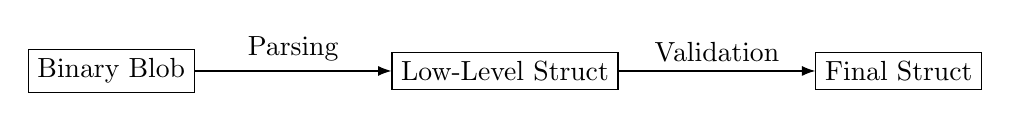
\begin{tikzpicture}
      \node[draw] (blob) at (0, 0) {Binary Blob};
      \node[draw] (ir) at (5, 0) {Low-Level Struct};
      \node[draw] (fin) at (10, 0) {Final Struct};

      \draw[-{LaTeX}] (blob) -- node[above]{Parsing} (ir);
      \draw[-{LaTeX}] (ir) -- node[above]{Validation} (fin);
    \end{tikzpicture}
    \caption{Progression from binary blob to fully parsed and validated struct.}
  \end{subfigure}

  \begin{subfigure}[b]{0.4\textwidth}
    \centering
    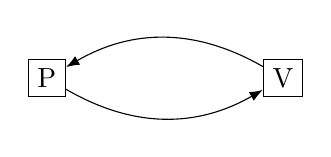
\begin{tikzpicture}
      \node[draw] (pp) at (0, 0) {P}; \node[draw] (pv) at (3, 0) {V};

      \draw[-{LaTeX}] (pp) edge[bend right] (pv); \draw[-{LaTeX}] (pv) edge[bend right] (pp);
    \end{tikzpicture}
    \caption{Protobuf parse validation loop for nested messages.}
  \end{subfigure}
  \hspace{1cm}
  \begin{subfigure}[b]{0.4\textwidth}
    \centering
    \begin{tikzpicture}
      \node[draw] (cp) at (0, 0) {P}; \node[draw] (cv) at (3, 0) {V};

      \draw[-{LaTeX}] (cp) -- (pv);
    \end{tikzpicture}
    \caption{CBOR parse validation flow. Tag 24 might require parsing again, but
    that is expected to be trigger by the host application at a later time.}
  \end{subfigure}

  \caption{Splitting the Protobuf and CDDL parse process into two steps, parsing
    and validating.}
  \label{fig:parse-validate}
\end{figure}

While I claimed earlier that Protobuf forces Pollux to consider the binary
encoding blob. Where is that expressed in any of the compatibility relations?
\emph{It's not.} Basically all of the existing work for Pollux on Protobuf can
be trivially lifted to operating on the protoscope level just by changing our
mental framing around it.

\section{Abstract State Schema}

In software verification, an implementation is always verified against some
specification of correct behavior. This is implicitly part of
\texttt{protobuf} too; when a message is serialized and transmitted over the
network, the developer expects that the same structure can be recreated by the
receiving program. Refactoring this intuition to be more directly applicable to
the standard verification setup, one could argue that the binary wire blob
serves as an ``implementation'' of the structure or object in the host
language (be it \texttt{go}, \texttt{java}, \texttt{python} or any other
language with \texttt{protobuf} bindings) which itself is generated by
\texttt{protoc} and is an ``implementation'' of the proto schema defined in a
\texttt{.proto} file. This stack defines the \texttt{.proto} file as the top
level source of truth, but this can be modeled by the high level host language
in most cases. From the prospective of an application developer, the host
language representation is the most important, since this is where the schema
structure interacts with other parts of the host application.

The definition of a \texttt{proto} message can be modeled by an \fstar{} type,
in a way similar to structures created by \texttt{protoc} for other host
languages. This is not fully sufficient though, since the representation
exposed by \texttt{protoc} isn't enough to fully reason about compatibility.

\subsection{\fstar{} Proto Struct Representation}

Some parts of the translation from a \texttt{proto} message
\autocite{LanguageGuideProto} into \fstar{} is simple. For example, a 64 bit
unsigned integer can be represented with a \texttt{UInt64} from the \fstar{}
machine integer library. Likewise a message can be represented by a record
\autocite{swamy2023proof}. Not everything cleanly generalizes
though. Specifically, it is unclear to how represent some primitive types such
as \texttt{float}, \texttt{double} or \texttt{string}.

\begin{table}[H]
	\centering
	\begin{tabular}{ll}
		\toprule
		\texttt{proto} Feature & \fstar{} Representation   \\
		\midrule
		Integers               & Machine Integer Library   \\
		\texttt{string}        & \texttt{string}           \\
		\texttt{message}       & Record                    \\
		\texttt{optional}      & \texttt{option}           \\
		\texttt{repeated}      & \texttt{list}             \\
		\texttt{map}           & ???                       \\
		\texttt{bool}          & \texttt{bool}             \\
		\texttt{bytes}         & \texttt{Seq.seq UInt8.t}  \\
		\texttt{enum}          & Inductive type            \\
		\texttt{oneof}         & Inductive type (Sum type) \\
		\texttt{option}        & ???                       \\
		\bottomrule
	\end{tabular}

	\vspace{4mm}
	\caption[]{\texttt{proto} language features and corresponding \fstar{} representations.}
\end{table}

Notice that there are several unknown representations in the table. Below is
some commentary on these features:

\begin{itemize}
	\item \texttt{map}: As far as I can tell, \fstar{} doesn't have maps, however
	      this \fstar{} development doesn't \emph{need} maps beyond a way to serialize
	      and de-serialize them. We should be able to develop a parametric
	      \texttt{map} definition as a list of tuples, just like how protobuf would
	      serialize them.
	\item \texttt{option}: This isn't an optional value, but rather top level
	      options used to set things like the \texttt{java} package. At the moment,
	      I'm not sure if or how changing values can impact protobuf compatibility.
\end{itemize}

A good completeness test might be encoding \texttt{descriptor.proto}, the proto
file which can encode other protobuf schema.

While this would provide a framework for building \fstar{} bindings for
protobuf, a richer representation for a protobuf schema for checking
compatibility at the wire level.

\subsection{Compatibility Checking with \fstar{} Types}

When a protobuf message is encoding, field names are stripped out in favor of
field numbers or field tags, which are manually defined in the protobuf
schema. Consider the two \texttt{proto} snippets below:

\begin{figure}[H]
	\centering
	\begin{minipage}[bt]{0.4\textwidth}
		\begin{lstlisting}[language=proto]
message Foo {
    int32 bar = 1;
}\end{lstlisting}
	\end{minipage}
	\hspace{1cm}
	\begin{minipage}[bt]{0.4\textwidth}
		\begin{lstlisting}[language=proto]
message Foo {
    int32 bar = 2;
}\end{lstlisting}
	\end{minipage}

	\caption[]{Example showing the importance of including proto field numbers in
		compatibility checking.}
\end{figure}

Any invocation of \texttt{protoc} will generate exactly the same
application-facing code, even though a message generated using the left proto
file will be parsed to an empty message by the right proto file.

This suggests that a more descriptive type is required. Rather than model the
struct that would be output by \texttt{protoc}, the source type for Pollux
should target the descriptor, as represented in the \texttt{.proto} file. Then,
in a manner similar to the \texttt{parse} function in Everparse, develop
something like this:

\begin{align*}
	\mathtt{Desc}               & : Type                                                                             \\
	\mathtt{Record}             & : Type \quad \text{Record corresponding to descriptor}                             \\
	\llbracket \cdot \rrbracket & : \mathtt{Desc} \rightarrow \mathtt{Record}                                        \\
	parse                       & : (d:\mathtt{Desc}) \rightarrow \mathtt{Bytes} \rightarrow option\
	\llbracket d \rrbracket                                                                                          \\
	serialize                   & : (d:\mathtt{Desc}) \rightarrow \llbracket d \rrbracket \rightarrow \mathtt{Bytes}
\end{align*}

Several shorthands arise from this, namely $parse_d : \mathtt{Bytes} \rightarrow option\
	\llbracket d \rrbracket$ for the partial application of a descriptor $d$ to
$parse$. The same thing can be done for $serialize_d : \llbracket d \rrbracket \rightarrow
	\mathtt{Bytes}$, which naturally to more traditional definitions of a parser and serializer.

\section{Protobuf Compatibility Questions}

As the \fstar{} development moves forward, it is beneficial to have a minimal
working example of a non-trivial compatibility question for protocol
buffers. There are several clearly trivial questions, like updating a
\texttt{int32} to an \texttt{int64} using the variable width integer encoding.

The protobuf encoding format is simple, which makes it challenging to construct
non-trivial compatibility question from small, trivial protobuf descriptions. As
an example, consider this example:

\begin{figure}[H]
	\centering
	\begin{minipage}[bt]{0.4\textwidth}
		\begin{lstlisting}[language=proto]
message Bar {
    string baz = 1;
}

message Foo {
    Bar bar = 1;
}\end{lstlisting}
	\end{minipage}
	\hspace{1cm}
	\begin{minipage}[bt]{0.4\textwidth}
		\begin{lstlisting}[language=proto]
message Foo {
    string bar = 1;
}\end{lstlisting}
	\end{minipage}

	\caption[]{A compatibility question.}
\end{figure}

The data is correctly exposed in the string on the right but there will be
several junk bytes at the beginning that the application has to trim. As a
definitional question, should this be considered compatible? Where or not a
client application can detect and correct the contents of the \texttt{bar} field
is beyond the current scope of this project.

From an encoding prospective, a protobuf message is encoded (mostly) as a
sequence of id, tag and value tuples. The id is the field number encoded in the
proto descriptor, the tag marks the type of value to follow and finally the
value contains the content set by the encoding application. More specifically,
the tag is from the table below.

\begin{table}[H]
	\centering
	\begin{tabular}{cll}
		\toprule
		ID & Name            & Uses                                                 \\
		\midrule
		0  & \texttt{VARINT} & \texttt{int32}, \texttt{int64}, \texttt{uint32},
		\texttt{uint64}, \texttt{sint32}, \texttt{sint64},
		\texttt{bool}, \texttt{enum}                                                \\
		1  & \texttt{I64}    & \texttt{fixed64}, \texttt{sfixed64}, \texttt{double} \\
		2  & \texttt{LEN}    & \texttt{string}, \texttt{bytes}, embedded messages,
		packed repeated fields                                                      \\
		5  & \texttt{I32}    & \texttt{fixed32}, \texttt{sfixed32},
		\texttt{float}                                                              \\
		\bottomrule
	\end{tabular}

	\vspace{4mm}
	\caption[]{Description of \texttt{proto} tag values. Note that values 3 and
		4 correspond to \texttt{SGROUP} and \texttt{EGROUP}, tags used in protobuf
		version 2 and deprecated in protobuf 3 \autocite{Encoding}.}\label{tab:tags}
\end{table}

It has finally become time for a sequence of definitions. A protobuf message
descriptor is comprised of a series of field descriptors, each of which has the
form \texttt{<<optional modifiers>> <<type>> <<field name>> = <<field
	number>>;}. During the encoding process, each field is encoded into an
encoding field, represented as tuple with 3 elements.
\\
\begin{definition}[Encoding Field]
	An encoding field is a tuple $(id, tag, value)$ which encodes the field
	number, tag and value of one field of a proto descriptor.
\end{definition}

Just like how the message descriptor is a sequence of field descriptors, the
encoding type of a message is an ordered list of encoding fields.
\\
\begin{definition}[Field Compatibility]
	For fields $f_1 = (id_1, tag_1, v_1)$ and $f_2 = (id_2, tag_2, v_2)$, $f_2$
	with descriptor $d_2$ is a compatible update to $f_1$ with descriptor $d_1$ if
	$id_1 = id_2$ and for all values $v_1$, $serialize_{d_1}\ f_1 = bs$ and there
	exists a $v_2$ such that $parse_{d_2}\ bs = v_2$ and $v_1 \prec v_2$ according to
	some relation $\prec$.
\end{definition}

An example value relation is given in Section~\ref{sec:val-rel}.
\\
\begin{definition}[Message Compatibility]
	A protobuf message descriptor $d_2$ is a compatible update to $d_1$ if every
	field in $d_1$ has a compatible field in $d_2$.
\end{definition}

Formally speaking, the message compatibility relation ($\preceq$) is given in
Section~\ref{sec:comp-rel}.
\\
\begin{definition}[Tag Function]
  The tag function $tag : \text{Type} \rightarrow \text{Tag}$ maps the \texttt{proto}
  level type to the corresponding tag as listed in Table~\ref{tab:tags}.
\end{definition}

It is also important to understand the default values of each protobuf
type. When a field is serialized with the default value or not set in the
message, the parser places the default value in the resulting struct. The
primary difference between an implicit field and an optional field is that the
optional field can differentiate between the serialized field being omitted from
the message or being present, but having the default value.
\\
\begin{definition}[Default Function]
  The default function
  $default: (t:\text{proto type}) \rightarrow \llbracket t \rrbracket$ returns the default
  value for each type.
  
  \[ default(t) = \left\{ 
    \begin{array}{l@{\quad:\quad}l}
      0 & t \in \left\{\begin{array}{c}
        \mathtt{int32}, \mathtt{int64}, \mathtt{uint32},
        \mathtt{uint64}, \mathtt{sint32}, \mathtt{sint64}, \\ \mathtt{fixed32},
        \mathtt{fixed64}, \mathtt{sfixed32}, \mathtt{sfixed64}, \mathtt{enum}
      \end{array}\right\} \\
      \mathtt{false} & t \text{ is } \mathtt{bool} \\
      ``" & t \text{ is } \mathtt{string} \\
      % 0 width space needed so that the brackets don't parse as a distance to
      % space out the elements of the array... for some unknown reason.
      \hspace{0pt}[\;] & t \text{ is } \mathtt{bytes}
    \end{array}\right.
  \]
\end{definition}


\section{Compatibility Relations}~\label{sec:comp-rel}

Compatibility between protobuf entities is defined with a series of
relations. The first and most self-contained relation is the value relation,
which relates two values at the specification level if serializing just a value
(such as a variable width integer) and then parsing it to a different protobuf
type would lead to a different value. After that is the protobuf type relation,
which relates two protobuf type is any value of the first type is related to
some value of the second type in the value relation. Since protobuf field and
message definitions will not have concrete values associated with them, the type
relation can be used in place of the value relation to make safe type
changes. Finally, the message relation connects compatible messages such that
all instances of the original message can be parsed into instances of the updated
message.

\subsection{Value Relation}~\label{sec:val-rel}

The value relation is the base level of the compatibility relations, relating
just two individual values. Protobuf values are modeled here as a specification
level type in \fstar{} associated with a protobuf type as listed in
Table~\ref{tab:val-spec}. Finally, while protobuf decorators are technically
part of the field level specification, they have been incorporated into the type
information to allow the specification type into include \texttt{option} or
\texttt{list} \fstar{} types.

\begin{table}[H]
	\centering
	\begin{tabular}{cl}
      \toprule
      Specification Type & Protobuf Type \\
      \midrule
      $\mathbb{Z}$ & \texttt{int32}, \texttt{uint32}, \texttt{sint32}
            \texttt{int64}, \texttt{uint64}, \texttt{sint64} \\
      $\mathbb{B}$ & \texttt{bool}    \\
      \texttt{string} & \texttt{string}    \\
      \texttt{list char}  & \texttt{bytes}    \\
      -- & \texttt{float}, \texttt{double} \\
      \bottomrule
	\end{tabular}

	\vspace{4mm}
	\caption[]{Description of the \fstar{} type corresponding to each protobuf
      type. Since \fstar{} doesn't support any type of floating point number,
      specification types cannot be provided for floating point protobuf types.}\label{tab:val-spec}
\end{table}

\begin{definition}[Value Relation]
  A protobuf value at the specification level $v_1$ with protobuf type $\tau_1$ is
  related to another value $v_2$ at type $\tau_2$, denoted $v_1 : \tau_1 \prec v_2 : \tau_2$
  if $parse_{\tau_2}\ serialize_{\tau_1}\ v_1 = v_2$.
\end{definition}

\subsubsection{Basic Rules}

The value relation is reflexive and transitive.

\begin{mathpar}
  \infer[Refl]{ }{v:\tau \prec v:\tau}

  \infer[Trans]{v_1:\tau_1 \prec v_2:\tau_2 \\ v_2:\tau_2 \prec v_3:\tau_3}{v_1:\tau_1 \prec v_3:\tau_3}
\end{mathpar}

\subsubsection{String \& Byte Rules}

It is possible to convert been the \texttt{string} and \texttt{bytes} types,
although the host program may have to deal with control character bytes being
present in the resulting string.

\begin{mathpar}
  \infer[Str-Byte]{ }{v : \mathtt{string} \prec v : \mathtt{bytes}}

  \infer[Byte-Str]{ }{v : \mathtt{bytes} \prec v : \mathtt{string}}
\end{mathpar}

\subsubsection{Integer Rules}

As a shorthand, statements like \texttt{uint[n]} represent a variable length
integer encoding into $n$ bits. In order to result in valid protobuf types, $n \in
\{32, 64\}$. The change width rules are designed to allow for both integer
promotion and demotion while the rest of the rules express what happens when
converting between integers using different encoding types for negative numbers.

With regard to the \textsc{Int-Chg-W} rule, I was originally concerned about
negative 32 bit numbers being encoded into 5 bytes for a varint encoding and
then becoming positive if parsed into 64 bit integer, but protobuf handles this
by writing all negative \texttt{int[n]} into a full 10 bytes. 

It is also worth noting that the expression $v : \tau$ actually refers to a value
of type $\llbracket \tau \rrbracket$ with a label of the type. All of the integer
types have $\llbracket \cdot \rrbracket = \mathbb{Z}$, as shown in Table~\ref{tab:val-spec},
which allows for the free conversion between integer types. Finally, $\%$ refers
to modulus using floored division, so $-1 \mod 2 = 1$ and the rules are
written with truncated integer division.

\begin{mathpar}
  \infer[Uint-Chg-W]{v_2 = v_1 \mod 2^m}{v_1 : \mathtt{uint[n]} \prec v_2 : \mathtt{uint[m]}}

  \infer[Int-Chg-W]{v_2 = (v_1 \mod 2^{m-1} - 2^{m-1} \times \mathbb{1}[v_1 < 0]}{v_1
    : \mathtt{int[n]} \prec v_2 : \mathtt{int[m]}}

  \infer[Sint-Chg-W]{v_2 = v_1 \mod 2^{m-1} - 2^{m-1} \times
    \mathbb{1}\left[\frac{v_1}{2^{m-1}} \mod 2 = 1\right]}{v_1 :
    \mathtt{sint[n]} \prec v_2 : \mathtt{sint[m]}}

  \infer[Uint-Int]{v_2 = v_1 - 2^n \times \mathbb{1}[v_1 \ge 2^{n-1}]}{v_1 :
    \mathtt{uint[n]} \prec v_2 : \mathtt{int[n]}}

  \infer[Int-Uint]{v_2 = v_1 + 2^n \times \mathbb{1}[v_1 < 0]}{v_1 :
    \mathtt{int[n]} \prec v_2 : \mathtt{uint[n]}} 

  \infer[Uint-Sint]{v_2 = (-1)^{v_1} \times \left( \frac{v_1}{2} \right) - (v_1 \%
    2)}{v_1 : \mathtt{uint[n]} \prec v_2 : \mathtt{sint[n]}} 

  \infer[Sint-Uint]{v_2 = 2 \times |v_1| - \mathbb{1}[v_1 < 0]}{v_1 :
    \mathtt{sint[n]} \prec v_2 : \mathtt{uint[n]}} 

  \infer[Int-Sint]
  {
    v_2 = \left\{
      {\begin{array}{l@{\quad:\quad}l}
        (-1)^{v_1} \times \left( \frac{v_1}{2} \right) - (v_1 \mod 2) & \text{if } v_1 \ge 0 \\
        (-1)^{v_1} \times \left(v_1 + 2^{n-1} - \frac{v_1}{2} \right) & \text{otherwise}
      \end{array}}\right.
  }
  {v_1 : \mathtt{int[n]} \prec v_2 : \mathtt{sint[n]}}

  \infer[Sint-Int]
  {
    v_2 = \left\{
      {\begin{array}{l@{\quad:\quad}l}
        2 \times |v_1| - \mathbb{1}[v_1 < 0] & \text{if } -2^{n-2} \le v_1 < 2^{n-2} \\
        2 \times |v_1| - 2^n - \mathbb{1}[v_1 < 0] & \text{otherwise}
      \end{array}}\right.
  }
  {v_1 : \mathtt{sint[n]} \prec v_2 : \mathtt{int[n]}}
\end{mathpar}

\subsubsection{Boolean Rules}

Booleans can be converted to and from any of the integer types.

\begin{mathpar}
  \infer[Uint-Bool]
  {
    v_2 = \left\{
      {\begin{array}{l@{\quad:\quad}l}
        \mathtt{false} & \text{if } v_1 = 0 \\
        \mathtt{true} & \text{otherwise}
      \end{array}}\right.
  }
  {v_1 : \mathtt{uint[n]} \prec v_2 : \mathtt{bool}}

  \infer[Bool-Uint]{v_2 = \mathbb{1}[v_1]}{v_1 : \mathtt{bool} \prec v_2 :
    \mathtt{uint[n]}} 

  \infer[Int-Bool]
  {
    v_2 = \left\{
      {\begin{array}{l@{\quad:\quad}l}
        \mathtt{false} & \text{if } v_1 = 0 \\
        \mathtt{true} & \text{otherwise}
      \end{array}}\right.
  }
  {v_1 : \mathtt{int[n]} \prec v_2 : \mathtt{bool}}

  \infer[Bool-Int]{v_2 = \mathbb{1}[v_1]}{v_1 : \mathtt{bool} \prec v_2 :
    \mathtt{int[n]}} 

  \infer[Sint-Bool]
  {
    v_2 = \left\{
      {\begin{array}{l@{\quad:\quad}l}
        \mathtt{false} & \text{if } v_1 = 0 \\
        \mathtt{true} & \text{otherwise}
      \end{array}}\right.
  }
  {v_1 : \mathtt{sint[n]} \prec v_2 : \mathtt{bool}}

  \infer[Bool-Sint]{v_2 = -\mathbb{1}[v_1]}{v_1 : \mathtt{bool} \prec v_2 :
    \mathtt{sint[n]}} 
\end{mathpar}

\subsubsection{Message \& Enum Rules}

Definitions for the structure of a message and enum are given in
Section~\ref{sec:msg-rel}. The values are represented as a mapping from the id
number of each field to the value and type of that field. 

\begin{mathpar}
  \infer[Msg]{\forall\ i \in ids(v_{m_2}).\ (i \in ids(v_{m_1}) \wedge v_i \prec v_i') \vee v_i' =
    default(\tau_i')}{v_{m_1} = \left\{ id_1:(v_1, \tau_1) \dots, id_n: (v_n, \tau_n)
    \right\} : \mathtt{MSG}\ m_1 \prec v_{m_2} = \left\{ id_1':(v_1', \tau_1') \dots,
      id_m':(v_m', \tau_m') \right\} : \mathtt{MSG}\ m_2}

  \infer[Enum]{v \in vals(e_2)}{v : \enum{s_1}{e_1} \prec v : \enum{s_2}{e_2}}
\end{mathpar}

\subsubsection{Decorator Rules}

Since the specification type can include \texttt{option}'s and \texttt{list}'s,
rules for handling these must also be present in the value relation. These rules
are grouped into introduction rules, which take implicit values and make them
optional or repeated, pass through rules which enable the above rules to operate
on these modified types.

{\color{red} There really should be a rule which can introduce a \texttt{None},
  but since implicit fields are modeled as just the spec type, this is
  difficult. I will likely need to model both implicit and optional fields with
  an \texttt{option}, add an annotation to the protobuf type and provide a
  function which introduces a default value for each type.}

\begin{mathpar}
  \infer[Rep-Pass]{v_1:\tau_1 \prec v_1':\tau_2 \\ \cdots \\ v_n:\tau_1 \prec v_n':\tau_2}{[v_1; \dots;
    v_n]: \rep{\tau_1} \prec [v_1'; \dots; v_n']: \rep{\tau_2}}

  \infer[Opt-Some-Pass]{v_1:\tau_1 \prec v_2:\tau_2}{(\some{v_1}): \opt{\tau_1} \prec
    (\some{v_2}): \opt{\tau_2}}

  \infer[Opt-None-Pass]{ }{\none: \opt{\tau_1} \prec \none: \opt{\tau_2}}
  
  \infer[Opt-Intro]{ }{v:\tau \prec (\some{v}): \opt{\tau}}

  \infer[Rep-Intro]{ }{v:\tau \prec [v]: \rep{\tau}}

  \infer[Missing-Imp]{ }{\none: \tau_1 \prec default(\tau_2):\tau_2}
\end{mathpar}

\subsection{Type Relation}~\label{sec:typ-rel}

This relation relates types which can be converted via the value relation.
\\
\begin{definition}[Type Relation]
  The type relation relates two protobuf type $\tau_1$ and $\tau_2$, denoted $\tau_1 \propto
  \tau_2$ if for all $v_1:\tau_1$ there exists a $v_2:\tau_2$ such that $v_1:\tau_1 \prec v_2:\tau_2$.
\end{definition}

\subsubsection{Base Type Rules}

\begin{mathpar}
  \infer[Str-Byt-T]{ }{\mathtt{string} \propto \mathtt{bytes}}

  \infer[Byt-Str-T]{ }{\mathtt{bytes} \propto \mathtt{string}}

  \infer[Int-Int-T]{\tau_1, \tau_2 \in \left\{{
        \begin{array}{c}
          \texttt{int32}, \texttt{int64}, \texttt{uint32}, \texttt{uint64} \\
          \texttt{sint32}, \texttt{sint64}, \texttt{bool}
        \end{array}
      }\right\}}{\tau_1 \propto \tau_2}
\end{mathpar}

\subsubsection{Message \& Enum Rules}

\begin{mathpar}
  \infer[Msg-T]{m_1 \preceq m_2}{\mathtt{MSG}\ m_1 \propto \mathtt{MSG}\ m_2}

  \infer[Enum-T]{vals(e_1) \subset vals(e_2)}{\enum{s_1}{e_1} \propto \enum{s_2}{e_2}}
\end{mathpar}

\subsubsection{Decorator Rules}

Since the type relation is designed for checking for safe type changes, it also
need to ensure that decorator restrictions like moving from a repeated field to
a singleton one aren't violated.

\begin{mathpar}
  \infer[Opt-Add-T]{ }{\tau \propto \opt{\tau}}

  \infer[Opt-Rm-T]{ }{\opt{\tau} \propto \tau}

  \infer[Opt-T]{\tau_1 \propto \tau_2}{\opt{\tau_1} \propto \opt{\tau_2}}

  \infer[Rep-Add-T]{ }{\tau \propto \rep{\tau}}

  \infer[Rep-T]{\tau_1 \propto \tau_2}{\rep{\tau_1} \propto \rep{\tau_2}}
\end{mathpar}

\subsection{Message Relation}~\label{sec:msg-rel}

The descriptor compatibility relation $\preceq$ is defined as below, but first it is
important to discuss the structure of fields and messages.

Each field is one of three different type of fields, the standard scalar field,
a map field or a \texttt{oneof} field. Specifically, the inductive type for
each style of field contains these pieces of information:

\begin{itemize}
\item \texttt{FIELD}: Contains the name of the field, the identifying field
  number and protobuf type (containing the decorator as well, possibly
  \texttt{OPT} or \texttt{REP}).
\item \texttt{MAP}: Contains the name of the field, the identifying field number
  and two protobuf types, one for the keys and one of the values.
\item \texttt{ONEOF}: Contains a name and a set of other fields.
\end{itemize}

A message descriptor and an enum descriptor are modeled one step above a field,
containing the following pieces of information:

\begin{itemize}
\item \texttt{MSG}: Contains the name of the message, a set of reserved indices
  and then a set of field definitions.
\item \texttt{ENUM}: Contains a set of name, id number pairs.
\end{itemize}

\subsubsection{Basic Rules}

A compatibility relation is both reflexive and transitive, although it is
neither symmetric nor anti-symmetric.  

\begin{mathpar}
   \infer[Refl-M]{ }{\msg{s}{r}{f} \preceq \msg{s}{r}{f}}

   \infer[Refl-E]{ }{\enum{s}{v} \preceq \enum{s}{v}}

   \infer[Trans-M]{\msg{s_1}{r_1}{f_1} \preceq \msg{s_2}{r_2}{f_2} \\
     \msg{s_2}{r_2}{f_2} \preceq \msg{s_3}{r_3}{f_3}}{\msg{s_1}{r_1}{f_1} \preceq
     \msg{s_3}{r_3}{f_3}}

   \infer[Trans-E]{\enum{s_1}{v_1} \preceq \enum{s_2}{v_2} \\
     \enum{s_2}{v_2} \preceq \enum{s_3}{v_3}}{\enum{s_1}{v_1} \preceq \enum{s_3}{v_3}}
\end{mathpar}

\subsubsection{Field Update Rules}

For the moment, names are recorded the protobuf field descriptors for accuracy
and to allow the relations to expand in the future. However, since names are
recorded in the encoded message, they are currently allowed to freely change.

\begin{mathpar}
  \infer[Field-Name]{ }{\msg{s_m}{r}{(f \cup \{\field{s_f}{id}{\tau}\})} \preceq
    \msg{s_m}{r}{(f \cup \{\field{s_f'}{id}{\tau}\})}}

  \infer[Map-Name]{ }{\msg{s_m}{r}{(f \cup \{\map{s_f}{id}{\tau_1}{\tau_2}\})} \preceq
    \msg{s_m}{r}{(f \cup \{\map{s_f'}{id}{\tau_1}{\tau_2}\})}}

  \infer[Oneof-Name]{ }{\msg{s_m}{r}{(f \cup \{\oneof{s_f}{f_o}\})} \preceq
    \msg{s_m}{r}{(f \cup \{\oneof{s_f'}{f_o}\})}}

  \infer[Field-Type]{\tau_1 \propto \tau_2}{\msg{s_m}{r}{(f \cup \{\field{s_f}{id}{\tau_1}\})} \preceq
    \msg{s_m}{r}{(f \cup \{\field{s_f}{id}{\tau_2}\})}}

  % TODO: May need restrictions about maps in maps...
  \infer[Map-Type-F]{\tau_1 \propto \tau_1' \\ \tau_2 \propto \tau_2' \\ \tau_1 \ne
    \mathtt{bytes}}{\msg{s_m}{r}{(f \cup \{\map{s_f}{id}{\tau_1}{\imp{\tau_2}}\})} \preceq
    \msg{s_m}{r}{(f \cup \{\map{s_f}{id}{\tau_1'}{\imp{\tau_2'}}\})}}
\end{mathpar}

\subsubsection{Oneof Rules}

The \texttt{oneof} rules are a bit complicated because a \texttt{oneof}
struggles against the notion that the field relations only connects one field to
one field by encapsulating several fields into a singular field.

\begin{mathpar}
  \infer[Oneof-Intro-Field]{m \in \{\mathtt{IMP}, \mathtt{OPT}\}}{\msg{s_m}{r}{(f
      \cup \{\field{s_f}{id}{(m\ \tau)}\})} \preceq \msg{s_m}{r}{(f \cup
      \{\oneof{s_o}{\{\field{s_f}{id}{(m\ \tau)}\}}\})}}

  % May need some statement about f_{n+1} not already being in the message?
  % You can introduce a new field, but not move an existing one.
  \infer[Oneof-Add-F]{m \in \{\mathtt{IMP}, \mathtt{OPT}\} \\ s_n \not \in names(f \cup
    f_o) \\ id_n \not \in ids(f \cup f_o)}{\msg{s_m}{r}{f \cup \{\oneof{s_f}{f_o}\}} \preceq
    \msg{s_m}{r}{f \cup \{\oneof{s_f}{(f_o \cup \{\field{s_n}{id_n}{(m\ \tau)}\})}\}}}

  % This rule should just be a combination of the above two rules...
  \infer[Oneof-Intro-New]{s_f \not \in names(f) \\ ids(f) \cap ids(f_o) = \emptyset \\
    names(f) \cap names(f_o) = \emptyset \\\\ \mathtt{REP} \not \in dec(f_o) \\ \forall f_n \in f_o.\
    f \ne \mathtt{MAP}}{\msg{s_m}{r}{f} \preceq \msg{s_m}{r}{(f \cup
      \{\oneof{s_f}{f_o}\})}}

  \infer[Oneof-Elim]{ }{\msg{s_m}{r}{(f \cup \{\oneof{s_f}{f_o}\})} \preceq \msg{s_m}{r}{(f
      \cup \{f_o\})}}

  % I'm not sure about the premise of this rule, but it seems better than having
  % to making another version of all the other rules. This is the first instance
  % where having a field relation would be very helpful.
  \infer[Oneof-Feild-Update]{\msg{``"}{\emptyset}{\{f\}} \preceq
    \msg{``"}{\emptyset}{\{f'\}}}{\msg{s}{r}{(f_m \cup \{\oneof{s_f}{(f_{o} \cup \{f\})}\})} \preceq
    \msg{s}{r}{(f_m \cup \{\oneof{s_f}{(f_o \cup \{f'\})}\})}}
\end{mathpar}

\subsubsection{Field \& Enum Rules}

Messages are similar to records in \fstar{} or other functional languages and
message compatibility can take the same two routes that record subtyping can:
width compatibility and depth compatibility. In width compatibility updates, new
fields are added to the message, making the updated version a strict superset of
the original message. In depth compatibility updates, the number of fields
remains the same, but other attributes of the field are updated compatible ways.

\begin{mathpar}
  \infer[Msg-Width-Field]{s_f \not \in names(f) \\ id \not \in
    ids(f)}{\msg{s_m}{r}{f} \preceq \msg{s_m}{r}{(f \cup \{\field{s_f}{id}{\tau}\})}}

  \infer[Msg-Width-Depth]{\msg{``"}{\emptyset}{\{f\}} \preceq
    \msg{``"}{\emptyset}{\{f'\}}}{\msg{s_m}{r}{(fs \cup \{f\})} \preceq
    \msg{s_m}{r}{(fs \cup \{f'\})}}
\end{mathpar}

The enum rules are similar to the message rules at least in the sense that enums
can be updated to have new fields without issue. However, when considering
removing fields from an enum definition, it is important to know if the enum is
treated as open or closed~\cite{EnumBehavior}. By default, \texttt{proto3}
treats all enums as open, so it should be possible to write a rule allowing for
the deletion of an enum field. This naturally aligns with how \texttt{go}
handles enums, since it doesn't support closed enums. Since protobuf enums don't
contain extra information, no depth rules is allowed.

\begin{mathpar}
  \infer[Enum-Width]{vals(e_1) \subset vals(e_2)}{\enum{s_1}{e_1} \preceq \enum{s_2}{e_2}}
\end{mathpar}

\subsubsection{Reserved Field Rules}

\begin{mathpar}
  \infer[Reserved-Add]{r \subset r'}{\msg{s}{r}{f} \preceq \msg{s}{r'}{f}}

  {\color{red}
    \infer[Reserved-Rm]{r \supset r'}{\msg{s}{r}{f} \preceq \msg{s}{r'}{f}}
  }
\end{mathpar}

\subsubsection{Valid Descriptors}

\begin{definition}[Valid Protobuf Descriptors]
  A protobuf message descriptor is \emph{valid}, denoted $v(d)$ if
  $\msg{``"}{\emptyset}{\emptyset} \preceq \msg{s}{r}{f}$.
\end{definition}

\subsubsection{Compatibility Theorem}

The main field-level compatibility theorem is stated below.
\\
\begin{theorem}[Field Compatibility]
  If $d_1 \preceq d_2$ then for all binary strings $bs$ such that
  $\mathtt{parse}_{d_1}\ bs = \mathtt{Some}\ v_1$, $\mathtt{parse}_{d_2}\ bs =
  \mathtt{Some}\ v_2$ and $v_1 \prec v_2$
\end{theorem}

\section{Adapting CBOR to Pollux}

Since the goal of Pollux is to start building a framework about general parser
compatibility (i.e.\ what happens if you parse with the wrong parser), it should
be general enough to express both protobuf and CBOR, as orthogonal as they
appear at the surface.

In the theory for protobuf, there are a number of relations at play. Briefly,
let's think about what each of the three relations would look like for CBOR:

\begin{itemize}
\item Value relation: Since each CBOR encoded value includes a header byte and
  argument (which in the case of an integer is actually the value of the
  integer, but for other types like text strings or byte strings would be the
  length of the string) before the value itself, we don't have the flexibility
  to slide values between types like we do in protobuf. Also, there is only one
  type of integer\ldots which is were most of the work on protobuf is focused. This
  relation would likely be nearly an identity relation with tagged values
  providing the most likely departure from an identity relation.
\item Compatible type relation: Like with the value relation, the one-to-one
  mapping from major types to base types in CDDL severely restricts the
  compatible type relation to be nearly an identity relation. However, once
  again tagged value and message types are likely to require some care.
\end{itemize}

Now, the above two points are \emph{possibly} lies. The presence of controls in
CDDL present an opportunity to add refinement types to the abstract value types,
in which case the value and type relations would grow in size (and complexity)
quite a bit. They would need to contain terms like
$5\ :\ \mathtt{int}\ .\mathtt{lt}\ 10 \prec 5\ :\ \mathtt{int}\ .\mathtt{lt}\ 15$
and $\mathtt{int}\ \mathtt{.lt}\ 10 \propto \mathtt{int}\ \mathtt{.lt}\ 15$. Note that
the value itself could never change, but the type can. The notation is a bit
clumsy, in my opinion, but comes directly from CDDL.

In both protobuf and CDDL, the final compatibility relation is still a
particular flavor of subtyping relation between message or map definitions. Each
of the two relations have points of complexity. In Protobuf, everything is
optional, allows for the addition of new fields which must obey the rules
defined by the protobuf language. CBOR on the other hand has required fields by
default, so the addition of new fields is limited to adding optional fields (and
maybe pulling a field out of a wildcard repeated field?) while there is much
more to think about with the refinement types that can be expressed in CDDL that
protobuf lacks.

\printbibliography{}
\end{document}

% Local Variables:
% citar-bibliography: ("./pollux.bib")
% TeX-command-default: "Make"
% jinx-local-words: "Everparse proto protobuf protoc protoscope"
% End:
